\documentclass[
    coverheight=9.249in,
    coverwidth=6.319in, % (pagesize - spinewidth) / 2
    spinewidth=1.125in,
    bleedwidth=0.306in,
    11pt,
    marklength=0pt,
  ]{bookcover}

  \usepackage{fancybox}
  \usepackage{wrapfig}
  \usepackage[many]{tcolorbox}
  \usetikzlibrary{calc,positioning, shadings}
  \usepackage[T1]{fontenc}
  \usepackage{fontspec}

  \setmainfont[
    Path=fonts/,
    Extension=.otf,
    UprightFont=*-Regular,
    ItalicFont=*-Italic,
    BoldFont=*-Bold,
    UprightFeatures={SmallCapsFont=*SC-Regular},
    ItalicFeatures={SmallCapsFont=*SC-Italic},
    BoldFeatures={SmallCapsFont=*SC-Bold},
    BoldItalicFeatures={SmallCapsFont=*SC-BoldItalic},
    ]{AlegreyaSans}

  \newcommand{\olpath}{../}
  \newcommand{\whitebg}[1]{%
  \tikz\node[circle,draw,minimum size=1.1cm,
  fill=white,
  path picture={
      \node at (path picture bounding box){
          \includegraphics[width=1.1cm]{\olpath#1}
      };
  }]{};
  }
  \newcommand{\bartosz}{
    \vspace{0pt}
    \begin{tcolorbox}[beamer,
      width=3.6cm,
      arc=0pt,
      boxsep=0pt,
      left=0pt,right=0pt,top=0pt,bottom=0pt,
      ] 
\includegraphics[width=3.6cm]{bartosz}
    \end{tcolorbox}
  }
  \newcommand\OPTversion{dev}

  \definecolor{BackgroundColor}{HTML}{f3f6ed}
  \definecolor{SpineBackColor}{HTML}{262626}

  \begin{document}

  \begin{bookcover}
    \bookcovercomponent{color}{bg whole}{color=BackgroundColor}
    \bookcovercomponent{color}{spine}{color=SpineBackColor}
    \bookcovercomponent{normal}{front}{
    % !TeX root = ./cover-paperback-reason.tex

\newcommand{\stripskip}{4}
\newcommand{\stripwidth}{3}

\definecolor{RedOrange}{rgb}{0.86, 0.30, 0.25}

\begin{tikzpicture}[
    overlay,
    remember picture,
    ribbon/.style={anchor=center, rotate = 45,
                            font={\fontsize{22}{1}\selectfont\bfseries}}
                    ]
    \coordinate (A) at ($ (current page.south east) + (-\stripskip,0) $);% <-- changed coordinate from 'north' to south'
    \coordinate (A') at ($(A) + (-\stripwidth,0) $);

    \coordinate (B) at ($ (current page.south east) + (0,\stripskip) $);% <-- changed coordinate from 'north' to south' and sign for \stripskip
    \coordinate (B') at ($(B) + (0,\stripwidth) $);% <-- changed sign for \stripskip

    \fill [RedOrange!20] (A) -- (A') -- (B') -- (B) -- cycle;

    \coordinate (tempA) at ($(A)!.5!(A')$);
    \coordinate (tempB) at ($(B)!.5!(B')$);

    \node [ribbon](text) at ($(tempA)!.5!(tempB)$) {
        \raisebox{-.15\height}{
\includegraphics[width=.8cm]{\olpath/fig/icons/reason}}
        \hspace{.5mm} ReasonML Edition
    };

\end{tikzpicture}
    \vspace{1.1cm}
    \begin{center}
      \fontsize{40pt}{5em}\selectfont\bfseries
          CATEGORY THEORY \\FOR PROGRAMMERS
      \vfil
      \hspace*{-.8cm}
\includegraphics[width=.5\coverwidth]{piggie}
      \linebreak
      \rule[1.5cm]{\textwidth/2}{.5pt}\\
      \vspace{-1.5cm}
      \normalfont\Huge\textbf{Bartosz Milewski}
      \vfil
      \vspace*{1cm}
    \end{center}}

    \bookcovercomponent{center}{spine}{
      \rotatebox[origin=c]{-90}{\color{orange}
      \Huge\bfseries Category Theory for Programmers \hspace{2em} Bartosz Milewski}}

    \bookcovercomponent{normal}{back}{%
    \begin{minipage}[b][\coverheight][t]{\coverwidth}
      \begin{center}
        \vspace{1cm}
        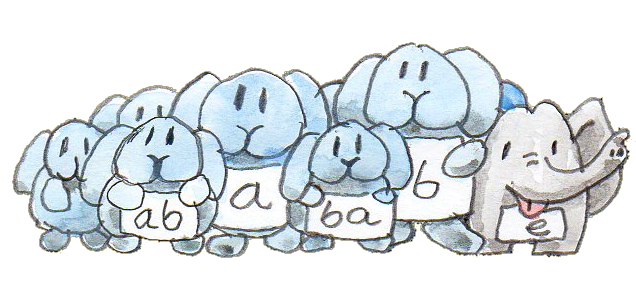
\includegraphics[width=.8\coverwidth]{bunnies}
        \begin{minipage}[t]{.8\coverwidth}
          % !TEX root = cover2.tex
% Blurb on back cover

{
\fontsize{16}{18.5}\selectfont
\lettrine[lhang=0.17]{C}{ategory Theory}
is one of the most abstract branches of mathematics. It is usually taught to
graduate students after they have mastered several other branches of mathematics,
like algebra, topology, and group theory. It might therefore come as a shock that
the basic concepts of category theory can be explained in relatively simple terms
to anybody with some experience in programming. \\

That's because, just like programming,
category theory is about structure. Mathematicians discover structure in mathematical
theories, programmers discover structure in computer programs. Well structured programs
are easier to understand and maintain, and are less likely to contain bugs. Category theory provides the language to talk about structure, and learning it will make you
a better programmer.
\vfil

}

          \vspace{.5cm}
        \end{minipage}

        \begin{minipage}{.85\textwidth}
          \rule{\textwidth}{.5pt}

          \begin{tabular}[h]{p{3.4cm} p{\textwidth}}
            \bartosz
            &
            \vspace{5pt}
            \begin{minipage}[b]{.58\coverwidth}
              \fontsize{11pt}{1.4em}\selectfont\textit{Category Theory for Programmers}
                is a series of blog posts by Bartosz Milewski, originally posted on bartoszmilewski.com.\\
                Edited by Igal Tabachnik. Licenced under CC BY-SA 4.0.\\
          \end{minipage}
        \end{tabular}
        \begin{flushright}
          \vspace{-2.6cm}
          \begin{minipage}[b]{4cm}
          \raggedleft
          \whitebg{fig/icons/by}
          \whitebg{fig/icons/cc}
          \whitebg{fig/icons/sa}
          \centering\footnotesize{\texttt{\OPTversion}}
          \end{minipage}
        \end{flushright}
      \end{minipage}
    \end{center}
  \end{minipage}
  }
  \end{bookcover}
\end{document}